% Digital position loop of a feed drive: block diagram
% (after Altintas, Manufacturing Automation)
\documentclass[dvisvgm,tikz,border=4pt]{standalone}
% Shared preamble for the TikZ figures in images-1/src (compiled by build.sh)
\usepackage{helvet}
\renewcommand\familydefault{\sfdefault}
\usepackage{amsmath, amssymb}
\usetikzlibrary{arrows.meta, calc, decorations.pathreplacing, patterns, positioning, shapes.geometric, 3d, perspective, fit, backgrounds}
% palette shared with slides.scss and the Graphviz diagrams
\definecolor{dmred}{HTML}{880000}
\definecolor{dmblue}{HTML}{000088}
\definecolor{dmgreen}{HTML}{008800}
\definecolor{dmorange}{HTML}{E08A1E}
\definecolor{ink}{HTML}{333333}
\definecolor{fillblue}{HTML}{E8E8F8}
\definecolor{fillred}{HTML}{F3EAEA}
\definecolor{fillgreen}{HTML}{E8F4E8}
\definecolor{fillorange}{HTML}{FDF0DC}
\definecolor{steel}{HTML}{C9D3DC}
\definecolor{steeldk}{HTML}{8FA3B5}
\definecolor{metal}{HTML}{D9D9D9}
\definecolor{metaldk}{HTML}{A6A6A6}
\tikzset{
  >={Stealth[length=7pt]},
  every picture/.style={line cap=round, line join=round, font=\large},
  proj/.style={gray, dashed, thin},
  dim/.style={<->, >={Stealth[length=5pt]}, thin},
  ext/.style={very thin, gray},
  callout/.style={gray!70!black, thin},
  % datum (origin) symbol
  % pics use absolute sizes so they look the same in mm-scaled drawings
  datum/.pic={
    \fill[white] (0,0) circle (0.22cm);
    \fill[black] (0,0) -- ++(0.22cm,0) arc[start angle=0, end angle=-90, radius=0.22cm] -- cycle;
    \fill[black] (0,0) -- ++(-0.22cm,0) arc[start angle=180, end angle=90, radius=0.22cm] -- cycle;
    \draw[thick] (0,0) circle (0.22cm);
  },
  % reference symbols (absolute sizes): origins have a double circle with a filled quadrant
  wporigin/.pic={
    \draw[thick, fill=white] (0,0) circle (0.3cm);
    \fill[black] (0,0) -- (0.18cm,0) arc[start angle=0, end angle=-90, radius=0.18cm] -- cycle;
    \draw[thick] (0,0) circle (0.18cm);
    \draw (-0.3cm,0) -- (0.3cm,0) (0,-0.3cm) -- (0,0.3cm);
  },
  machorigin/.pic={
    \draw[thick, fill=white] (0,0) circle (0.3cm);
    \fill[black] (0,0) -- (-0.18cm,0) arc[start angle=180, end angle=90, radius=0.18cm] -- cycle;
    \draw[thick] (0,0) circle (0.18cm);
    \draw (-0.3cm,0) -- (0.3cm,0) (0,-0.3cm) -- (0,0.3cm);
  },
  supportpt/.pic={
    \draw[thick, fill=white] (0,0) circle (0.15cm);
    \draw (-0.15cm,0) -- (0.15cm,0) (0,-0.15cm) -- (0,0.15cm);
  },
  regpt/.pic={
    \draw[thick, fill=white] (0,0) circle (0.24cm);
    \draw[thick] (0,0) circle (0.15cm);
    \draw (-0.15cm,0) -- (0.15cm,0) (0,-0.15cm) -- (0,0.15cm);
  },
  % support / registration point (generic)
  target/.pic={
    \draw[thick, fill=white] (0,0) circle (0.12cm);
    \draw (-0.2cm,0) -- (0.2cm,0) (0,-0.2cm) -- (0,0.2cm);
  },
}

% Shared style for the control block diagrams (not compiled on its own)
\definecolor{blockfill}{HTML}{F9F9FF}
\tikzset{
  ctl/.style={>={Stealth[length=6pt]}, line width=0.8pt, font=\large},
  block/.style={draw=ink!80, fill=blockfill, minimum height=1cm, minimum width=2cm,
                align=center, inner sep=5pt},
  hblock/.style={block, draw=dmred, fill=fillred, text=dmred},
  cblock/.style={block, draw=dmblue, fill=fillblue},
  sum/.style={circle, draw=ink!80, fill=white, minimum size=0.45cm, inner sep=0pt},
  branch/.style={circle, fill=ink, inner sep=0pt, minimum size=4.5pt},
  sig/.style={->},
  mech/.style={double=white, double distance=2.4pt, line width=0.7pt},
  lbl/.style={font=\normalsize, inner sep=2pt},
  group/.style={draw=#1, dashed, rounded corners=8pt, inner sep=12pt},
  grouplabel/.style={font=\normalsize\bfseries, text=#1, anchor=north west, inner sep=4pt},
}
% \sign{sum node}{angle}{sign}: + or - next to the input of a summing junction
\newcommand\sign[3]{\node[font=\normalsize, inner sep=0pt] at ($(#1)+(#2:0.48)$) {$#3$};}

\begin{document}
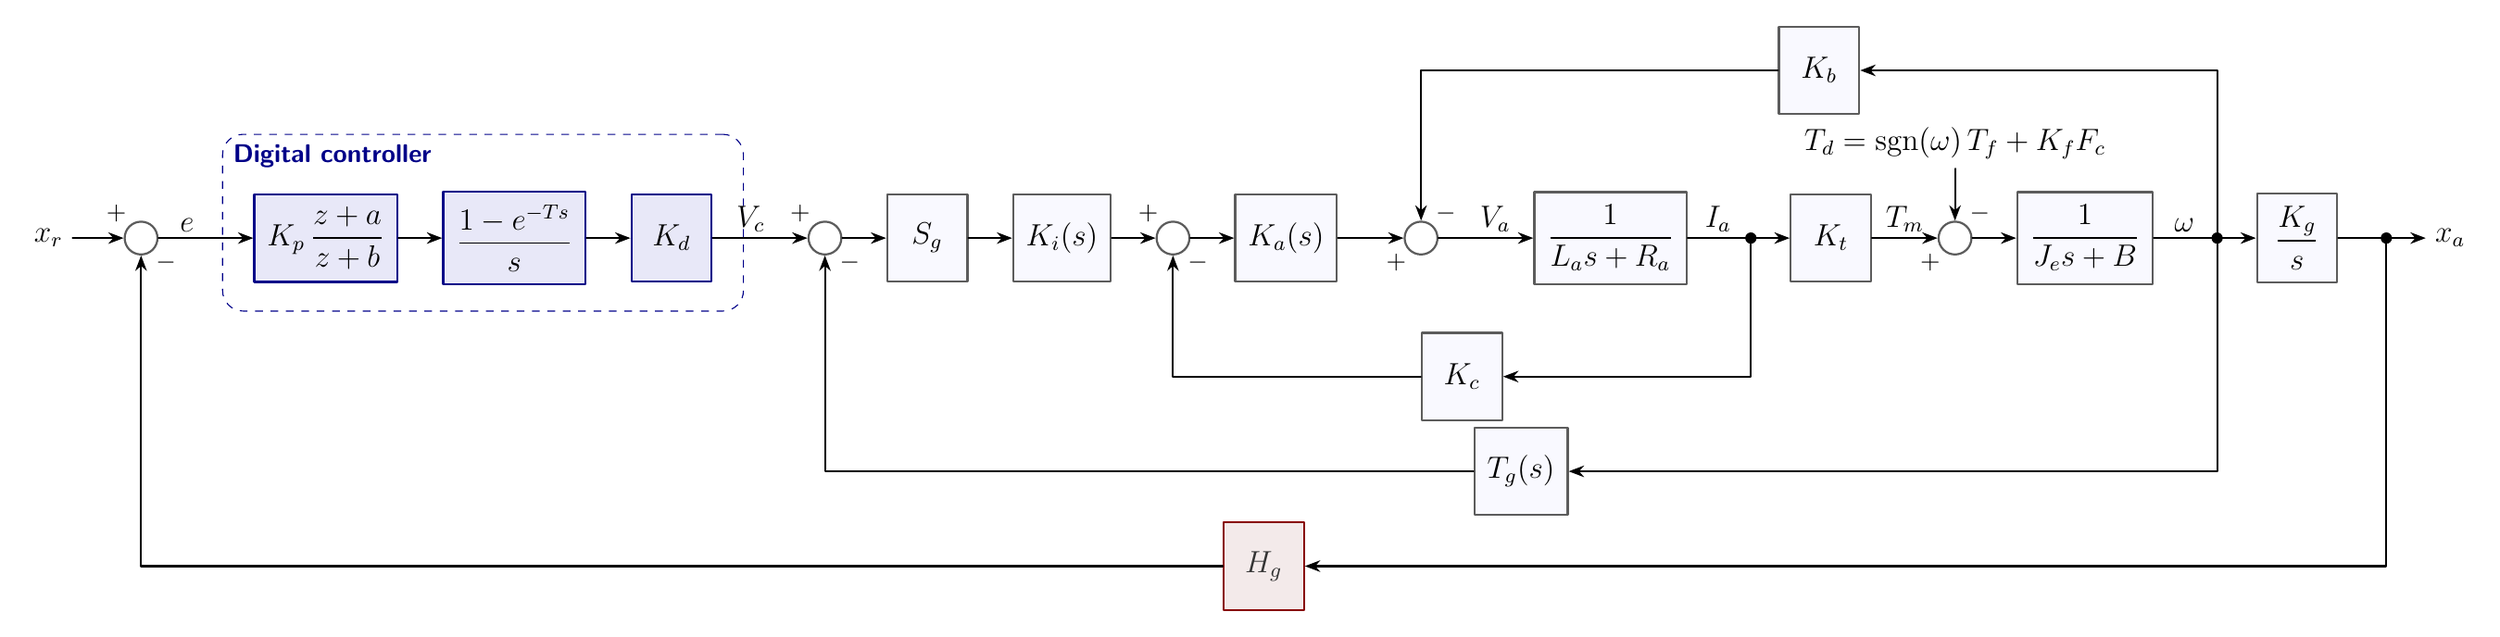
\begin{tikzpicture}[ctl, node distance=0.6cm,
    block/.append style={minimum width=1.1cm, minimum height=1.2cm},
    s/.style={above, inner sep=2pt}]
  % main row
  \node (xr) {$x_r$};
  \node[sum, right=0.7cm of xr] (s1) {};
  \node[cblock, right=1.3cm of s1] (filt) {$K_p\,\dfrac{z+a}{z+b}$};
  \node[cblock, right=of filt] (zoh) {$\dfrac{1-e^{-Ts}}{s}$};
  \node[cblock, right=of zoh] (kd) {$K_d$};
  \node[sum, right=1.3cm of kd] (s2) {};
  \node[block, right=of s2] (sg) {$S_g$};
  \node[block, right=of sg] (ki) {$K_i(s)$};
  \node[sum, right=of ki] (s3) {};
  \node[block, right=of s3] (ka) {$K_a(s)$};
  \node[sum, right=0.9cm of ka] (s4) {};
  \node[block, right=1.3cm of s4] (ele) {$\dfrac{1}{L_a s+R_a}$};
  \node[block, right=1.4cm of ele] (kt) {$K_t$};
  \node[sum, right=0.9cm of kt] (s5) {};
  \node[block, right=of s5] (mec) {$\dfrac{1}{J_e s+B}$};
  \node[block, right=1.4cm of mec] (kg) {$\dfrac{K_g}{s}$};
  \node[right=1.2cm of kg] (xa) {$x_a$};
  \coordinate (t1) at ($(ele.east)!0.62!(kt.west)$);
  \coordinate (t2) at ($(mec.east)!0.62!(kg.west)$);
  \coordinate (t3) at ($(kg.east)!0.55!(xa.west)$);
  % feedback blocks
  \node[block] (kc) at ($(s3)!0.5!(t1)+(0,-1.9)$) {$K_c$};
  \node[block] (kb) at ($(s4)!0.5!(t2)+(0,2.3)$) {$K_b$};
  \node (td) at ($(s5)+(0,1.3)$) {$T_d=\operatorname{sgn}(\omega)\,T_f+K_f F_c$};
  \node[block] (tg) at ($(s2)!0.5!(t2)+(0,-3.2)$) {$T_g(s)$};
  \node[hblock, text=ink] (hg) at ($(s1)!0.5!(t3)+(0,-4.5)$) {$H_g$};
  \begin{scope}[on background layer]
    \node[group=dmblue, fit=(filt) (zoh) (kd), inner ysep=16pt, yshift=6pt] (pc) {};
  \end{scope}
  \node[grouplabel=dmblue] at (pc.north west) {Digital controller};
  % forward path
  \draw[sig] (xr) -- (s1);
  \draw[sig] (s1) -- node[s, pos=0.3] {$e$} (filt);
  \draw[sig] (filt) -- (zoh);
  \draw[sig] (zoh) -- (kd);
  \draw[sig] (kd) -- node[s, pos=0.4] {$V_c$} (s2);
  \draw[sig] (s2) -- (sg);
  \draw[sig] (sg) -- (ki);
  \draw[sig] (ki) -- (s3);
  \draw[sig] (s3) -- (ka);
  \draw[sig] (ka) -- (s4);
  \draw[sig] (s4) -- node[s, pos=0.6] {$V_a$} (ele);
  \draw[sig] (ele) -- node[s, pos=0.3] {$I_a$} (kt);
  \draw[sig] (kt) -- node[s] {$T_m$} (s5);
  \draw[sig] (s5) -- (mec);
  \draw[sig] (mec) -- node[s, pos=0.3] {$\omega$} (kg);
  \draw[sig] (kg) -- (xa);
  % feedback paths
  \fill (t1) circle (2.2pt) (t2) circle (2.2pt) (t3) circle (2.2pt);
  \draw[sig] (t1) |- (kc.east);
  \draw[sig] (kc.west) -| (s3.south);
  \draw[sig] (t2) |- (kb.east);
  \draw[sig] (kb.west) -| (s4.north);
  \draw[sig] (td) -- (s5.north);
  \draw[sig] (t2) |- (tg.east);
  \draw[sig] (tg.west) -| (s2.south);
  \draw[sig] (t3) |- (hg.east);
  \draw[sig] (hg.west) -| (s1.south);
  \foreach \s in {s1, s2, s3} {\sign{\s}{135}{+} \sign{\s}{-45}{-}}
  \sign{s4}{-135}{+} \sign{s4}{45}{-}
  \sign{s5}{-135}{+} \sign{s5}{45}{-}
\end{tikzpicture}
\end{document}
